\documentclass[aspectratio=169,10pt]{beamer}

\usetheme[progressbar=frametitle]{metropolis}
\usepackage{appendixnumberbeamer}

\usepackage{booktabs}
\usepackage[scale=2]{ccicons}

\usepackage{pgfplots}
\usepgfplotslibrary{dateplot}

\usepackage{xspace}
\newcommand{\themename}{\textbf{\textsc{metropolis}}\xspace}

\usepackage[spanish,es-tabla]{babel}

\usepackage{xcolor}
\definecolor{dkgreen}{rgb}{0,0.6,0}
\definecolor{gray}{rgb}{0.5,0.5,0.5}
\definecolor{mauve}{rgb}{0.58,0,0.82}
\usepackage{listings}
\lstset{%
	numberstyle=\tiny,
	basicstyle=\fontsize{6}{8}\ttfamily,
	numbersep=15pt,tabsize=4,
	flexiblecolumns=true,
	keywordstyle=\color{blue},
	commentstyle=\color{dkgreen},
	stringstyle=\color{mauve},
	numberstyle=\tiny\color{gray},
	language=Java,
	breaklines=true,
	breakatwhitespace=true,
  showstringspaces=false,
  aboveskip=0.1em,
  belowskip=0.5em,
	morekeywords={*,num,String,var,library,get,set,StringEq,StringHashEq,bool,Top,Bot,<,String@L,String@H,int@L,int@H} ,
}


\title{DESCLASIFICACIÓN BASADA EN TIPOS EN DART}
\subtitle{IMPLEMENTACIÓN Y ELABORACIÓN DE HERRAMIENTAS DE INFERENCIA}
% \date{\today}
\date{}
\author{Matías Meneses Cortés}
%\institute{Departamento de Ciencias de la Computación}
\titlegraphic{\hfill
\includegraphics[height=2.5cm]{logo.png}}

\begin{document}

\maketitle

\begin{frame}{Contenidos}
  \setbeamertemplate{section in toc}[sections numbered]
  \tableofcontents[hideallsubsections]
\end{frame}

\section{Control de flujo de información}

\begin{frame}[fragile]{Protección de confidencialidad}
  \begin{center}
    \only<1>{
\includegraphics[width=0.8\textwidth]{images/interaccion.png}}
    \only<2>{
\includegraphics[width=0.8\textwidth]{images/interaccion2.png}}
  \end{center}
\end{frame}

\begin{frame}[fragile]{Protección de confidencialidad}
  Distintas técnicas de seguridad en distintas capas de comunicación. \pause
  \vspace{0.5cm}
  \begin{columns}[T,onlytextwidth]
    \column{0.6\textwidth}
    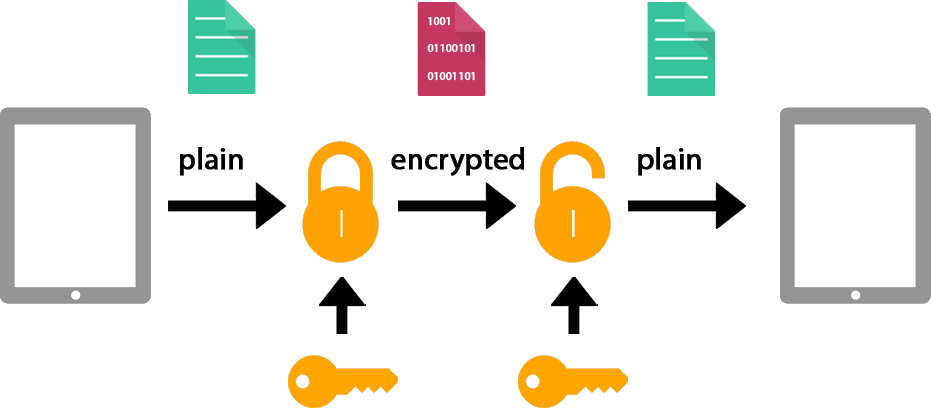
\includegraphics[width=0.8\textwidth]{images/e2e.png} \pause
    \column{0.4\textwidth}
    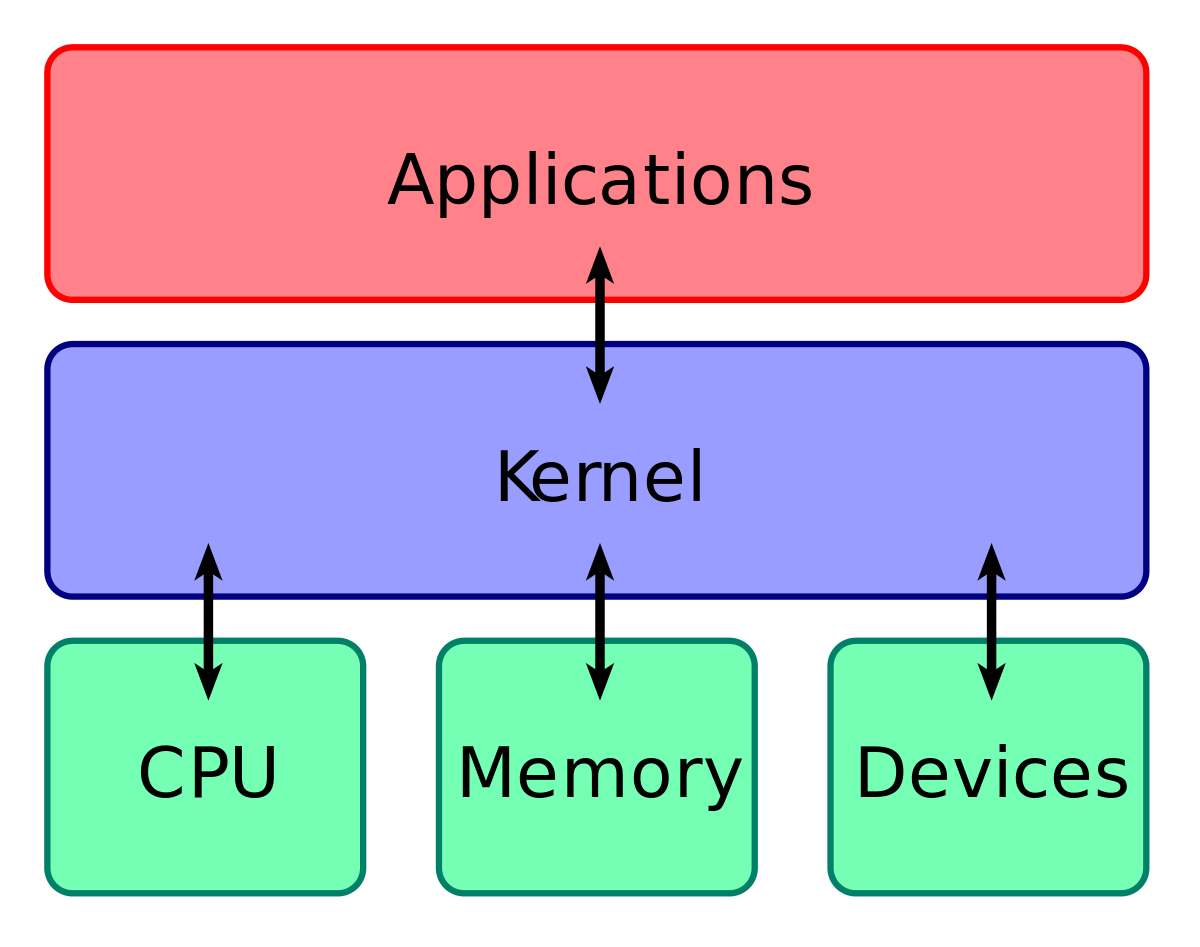
\includegraphics[width=1.0\textwidth]{images/kernel.png}
  \end{columns}
\end{frame}

\begin{frame}[fragile]{Seguridad basada en el lenguaje}
  \begin{center}
    
\includegraphics[width=0.4\textwidth]{images/lbs.png}
  \end{center}
\end{frame}

\begin{frame}[fragile]{Control de flujo de información}
  \begin{columns}[T,onlytextwidth]
    \column{0.3\textwidth}
    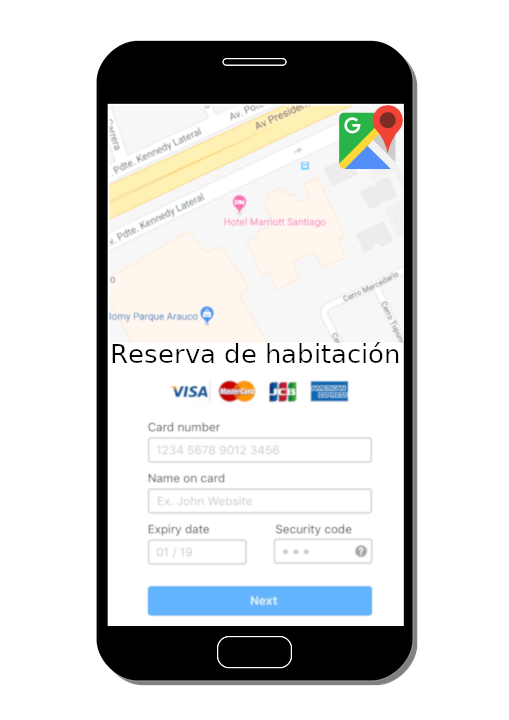
\includegraphics[width=1.0\textwidth]{images/book.png}
    \column{0.7\textwidth}
    \vspace{1cm}
    \begin{onlyenv}<1>
      \begin{lstlisting}
        String book(String username, int date, int cardNumber) {
          return sendToHotel(username, date, cardNumber);
        }

        String sendToHotel(String username, int date, int cardNumber);
        String sendToGoogle(String token, int xCoord, int yCoord);
      \end{lstlisting}
    \end{onlyenv}
    \begin{onlyenv}<2>
      \begin{lstlisting}[escapechar=?]
        String book(String username, int date, int cardNumber) {
          return ?\colorbox{yellow!50}{sendToGoogle}?(username, date, cardNumber);
        }

        String sendToHotel(String username, int date, int cardNumber);
        String sendToGoogle(String token, int xCoord, int yCoord);
      \end{lstlisting}
    \end{onlyenv}

  \end{columns}
\end{frame}

\begin{frame}[fragile]{Tipado de seguridad para el control de flujo de información}

  \begin{columns}[T,onlytextwidth]
    \column{0.3\textwidth}
    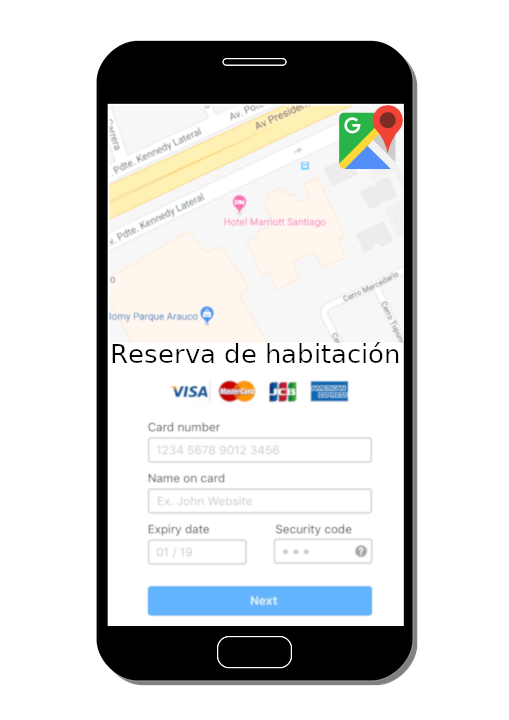
\includegraphics[width=1.0\textwidth]{images/book.png}
    \column{0.7\textwidth}
    \vspace{1cm}
    \begin{onlyenv}<1>
      \begin{lstlisting}
        String@L book(String@L username, int@L date, int@H cardNumber) {
          return sendToGoogle(username, date, cardNumber);
        }

        String@L sendToHotel(String@L username, int@L date, int@H cardNumber);
        String@L sendToGoogle(String@H token, int@L xCoord, int@L yCoord);
      \end{lstlisting}
    \end{onlyenv}
    \begin{onlyenv}<2>
      \begin{lstlisting}[escapechar=?]
        String@L book(String@L username, int@L date, int@H cardNumber) {
          ?\colorbox{red!20}{return sendToGoogle(username, date, cardNumber);}?
        }

        String@L sendToHotel(String@L username, int@L date, int@H cardNumber);
        String@L sendToGoogle(String@H token, int@L xCoord, int@L yCoord);
      \end{lstlisting}
    \end{onlyenv}
  \end{columns}

\end{frame}

\begin{frame}[fragile]{No-interferencia}
  Propiedad fundamental del control de flujo de información.
	\begin{center}
		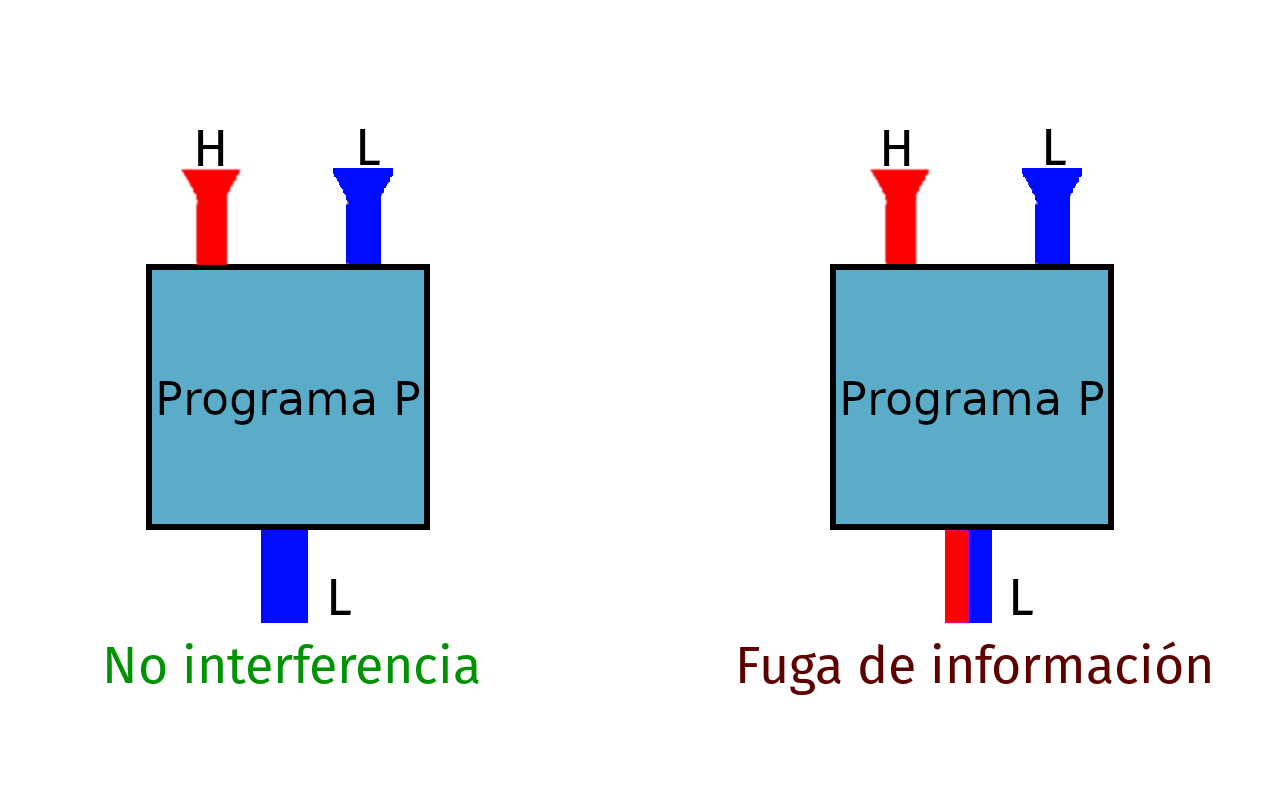
\includegraphics[width=0.8\textwidth]{images/noninterference.png}
	\end{center}

\end{frame}

\begin{frame}[fragile]{Detección de flujos explícitos inválidos}
	\begin{columns}[T,onlytextwidth]
		\column{0.33\textwidth}
		(asignación) \pause
		\column{0.33\textwidth}
		(argumento y parámetro) \pause
		\column{0.33\textwidth}
		(retorno)
	\end{columns}
\end{frame}

\begin{frame}[fragile]{Detección de flujos implícitos inválidos}
	\begin{columns}[T,onlytextwidth]
		\column{0.65\textwidth}
		\begin{onlyenv}<1>
			(codigo con if)
		\end{onlyenv}
		\begin{onlyenv}<2>
			(codigo con if y marca de pc)
		\end{onlyenv}
		\column{0.35\textwidth}

		\only<2>{Contexto de seguridad (\alert{\texttt{pc}}).}
	\end{columns}
\end{frame}

\begin{frame}[fragile]{Problema con no-interferencia}
	\begin{center}
		(Código de login) \pause \\
		\vspace{4cm}
		\alert{¡\textbf{No} cumple con no-interferencia!}
	\end{center}
\end{frame}

\begin{frame}[fragile]{Desclasificación}
	\begin{center}
		(Código de login con declassify)
	\end{center}
\end{frame}

\begin{frame}[fragile]{Problema con desclasificación}
	\begin{center}
		(Código de login con declassify(password)) \pause \\
		\vspace{4cm}
		\alert{¡Grave fuga de información!}
	\end{center}
\end{frame}

\begin{frame}[fragile]{Desclasificación basada en tipos}
	\begin{columns}[T,onlytextwidth]
		\column{0.6\textwidth}
		(código con tipos de dos facetas)
		\column{0.4\textwidth}
		\begin{itemize}
			\item \texttt{StringEq =} \\ \texttt{[eq: String -> Bool]}
			\item \texttt{String <: StringEq} \\ (Tipo bien formado)
			\item No-interferencia relajada
		\end{itemize}
	\end{columns}
\end{frame}

\begin{frame}[fragile]{Retículo de subtipos}
	\begin{center}
		(figura de reticulo)
	\end{center}
\end{frame}

\begin{frame}[fragile]{Reglas principales de la desclasificación basada en tipos}
	\begin{columns}[T,onlytextwidth]
		\column{0.5\textwidth}
		(código)
		\column{0.5\textwidth}
		\metroset{block=fill}
		\begin{block}{Métodos autorizados (TmD)}
			(regla formal)
		\end{block}
	\end{columns}
\end{frame}

\begin{frame}[fragile]{Reglas principales de la desclasificación basada en tipos}
	\begin{columns}[T,onlytextwidth]
		\column{0.5\textwidth}
		(código)
		\column{0.5\textwidth}
		\metroset{block=fill}
		\begin{block}{Métodos no autorizados (TmH)}
			(regla formal)
		\end{block}
	\end{columns}
\end{frame}

\begin{frame}[fragile]{Problemas con la desclasificación basada en tipos}
	\begin{itemize}
		\item Propuesta sin implementación práctica. \pause
		\item Anotación completa de facetas para realizar análisis. \pause
	\end{itemize}

	\begin{onlyenv}<3>
		(código con facetas públicas anotadas)
	\end{onlyenv}
	\begin{onlyenv}<4>
		(código sin facetas públicas anotadas)
	\end{onlyenv}
\end{frame}

\section{Inferencia de tipos}

\begin{frame}[fragile]{Inferencia de tipos}
	\begin{onlyenv}<1>
		(codigo con anotaciones de tipo)
	\end{onlyenv}
	\begin{onlyenv}<2>
		(codigo parcialmente anotado)
	\end{onlyenv}
\end{frame}

\begin{frame}[fragile]{Variables de tipo}
	(codigo anotado con variables de tipo)
\end{frame}

\begin{frame}[fragile]{Generación de restricciones}
	\begin{columns}[T,onlytextwidth]
		\column{0.6\textwidth}
		(codigo anotado con variables de tipo)
		\column{0.4\textwidth}
		(restricciones generadas)
	\end{columns}
\end{frame}

\begin{frame}[fragile]{Resolución de restricciones}
	(Mostrar substituciones hasta resolver)
\end{frame}

\begin{frame}[fragile]{Restricciones sobre subtipos}
	\begin{columns}[T,onlytextwidth]
		\column{0.6\textwidth}
		(codigo anotado con variables de tipo) \\
		\only<1>{(retículo de subtipos)}
		\only<2>{(retículo de subtipos mostrando meet y join)}
		\column{0.4\textwidth}
		(restricciones generadas)
	\end{columns}
\end{frame}

\begin{frame}[fragile]{Objetivo de la memoria}
	\metroset{block=fill}
	\begin{block}{Objetivo de la memoria}
		Implementar un sistema de inferencia de facetas públicas para la desclasificación basada en tipos, en conjunto con una extensión para ambientes de desarrollo.
	\end{block}
\end{frame}

\section{Inferencia de facetas públicas en Dart}

\begin{frame}[fragile]{Lenguaje Dart}
	\begin{center}
		
\includegraphics[width=0.75\textwidth]{images/dart.png}
	\end{center}
\end{frame}

\begin{frame}[fragile]{Dart Analyzer}
	\begin{center}
		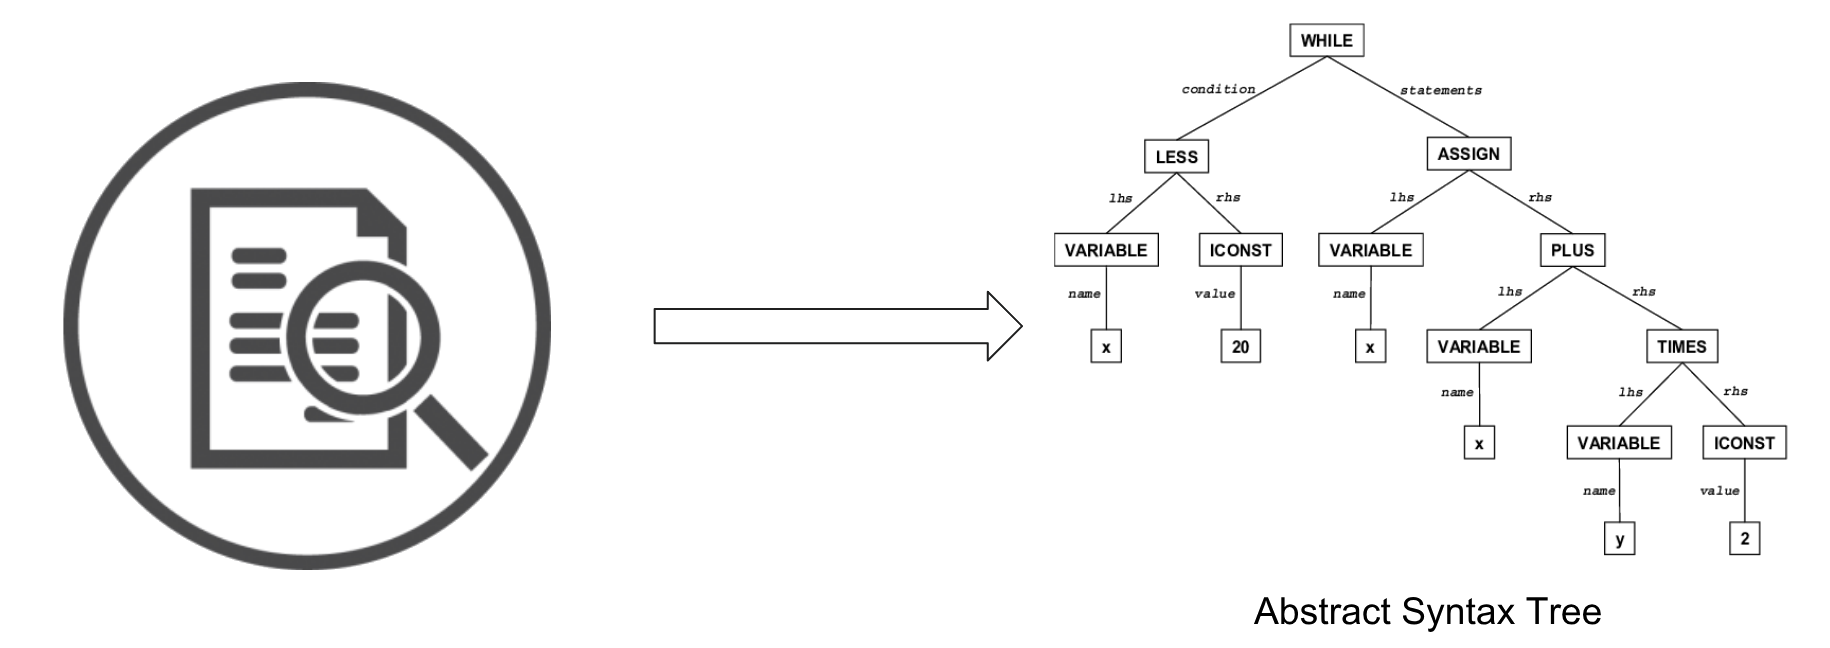
\includegraphics[width=1.0\textwidth]{images/ast.png}
	\end{center}
\end{frame}

\begin{frame}[fragile]{Analyzer Plugin}
		\begin{center}
			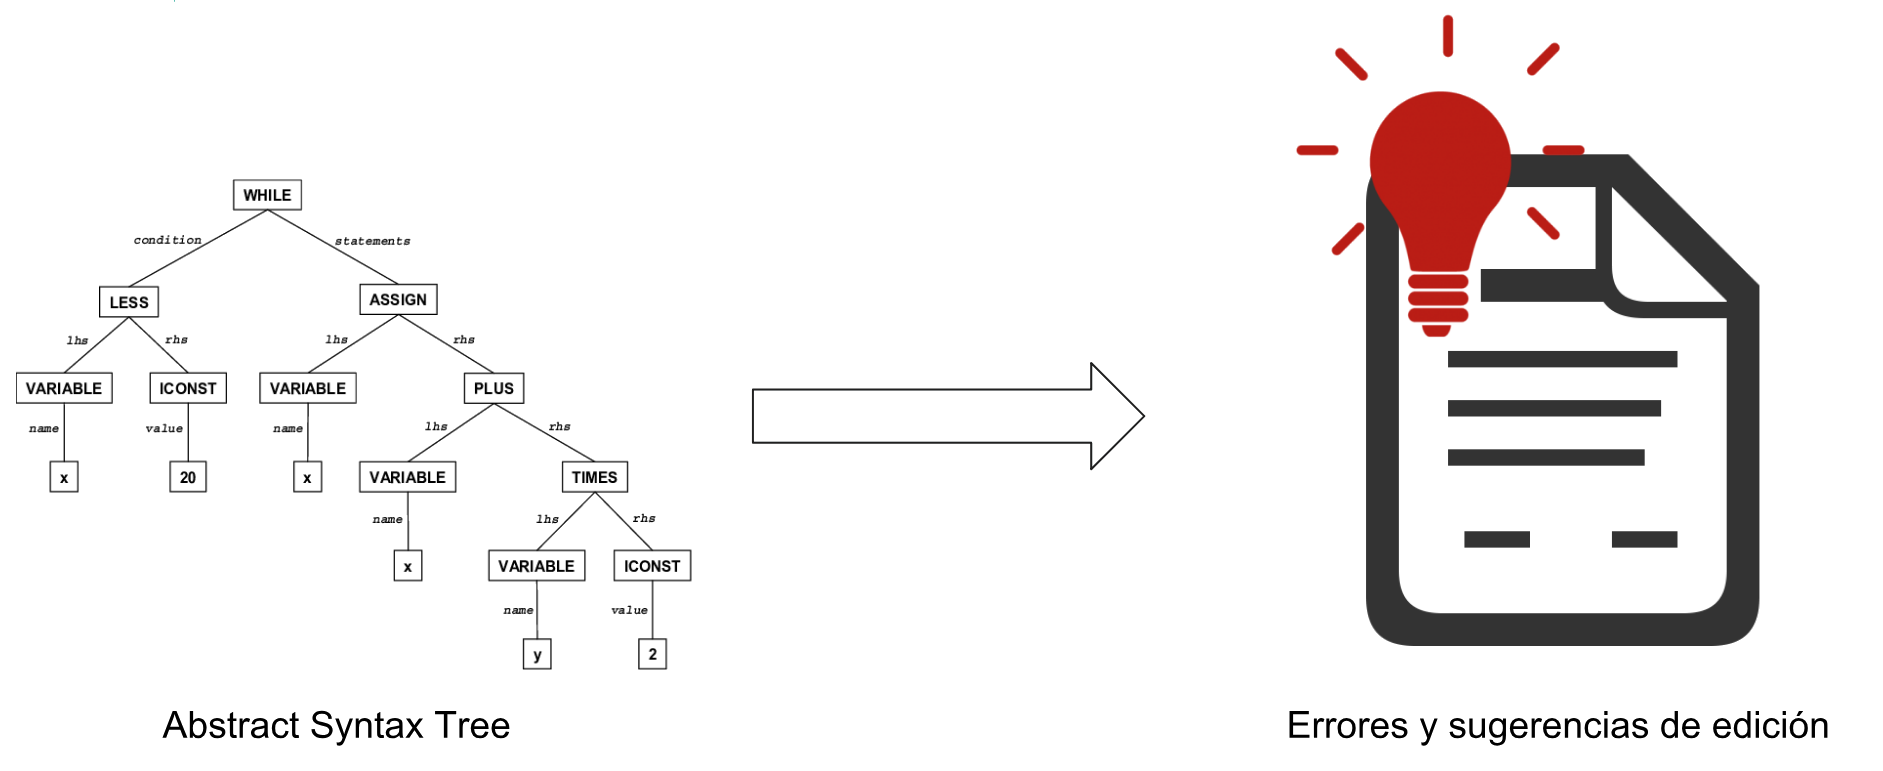
\includegraphics[width=1.0\textwidth]{images/plugin.png}
		\end{center}
\end{frame}

\begin{frame}[fragile]{Problema de inferencia a resolver}
	\metroset{block=fill}
	\begin{block}{Problema de inferencia}
		Dado un programa Dart parcialmente tipado con facetas públicas, y completamente tipado con facetas privadas, encontrar la faceta pública de las expresiones no tipadas que más se ajuste al uso de las expresiones, tal que el programa sea bien tipado.
	\end{block} \pause
	\begin{onlyenv}<2>
		(código parcialmente tipado 1)
	\end{onlyenv}
	\begin{onlyenv}<3>
		(código con tipos inferidos 1)
	\end{onlyenv}
\end{frame}
\begin{frame}[fragile]{Problema de inferencia a resolver}
	\metroset{block=fill}
	\begin{block}{Problema de inferencia}
		Dado un programa Dart parcialmente tipado con facetas públicas, y completamente tipado con facetas privadas, encontrar la faceta pública de las expresiones no tipadas que más se ajuste al uso de las expresiones, tal que el programa sea bien tipado.
	\end{block}
	\begin{onlyenv}<1>
		(código parcialmente tipado 2)
	\end{onlyenv}
	\begin{onlyenv}<2>
		(código con tipos inferidos 2)
	\end{onlyenv}
\end{frame}
\begin{frame}[fragile]{Problema de inferencia a resolver}
	\metroset{block=fill}
	\begin{block}{Problema de inferencia}
		Dado un programa Dart parcialmente tipado con facetas públicas, y completamente tipado con facetas privadas, encontrar la faceta pública de las expresiones no tipadas que más se ajuste al uso de las expresiones, tal que el programa sea bien tipado.
	\end{block}
	\begin{onlyenv}<1>
		(código parcialmente tipado 3)
	\end{onlyenv}
	\begin{onlyenv}<2>
		(código con tipos inferidos 3)
	\end{onlyenv}
\end{frame}

\begin{frame}[fragile]{Pasos de la solución}
	\begin{enumerate}
		\item Definición del subconjunto de Dart soportado.
		\item Definición y declaración de facetas públicas en Dart.
		\item Integración de tipos estáticos comunes de Dart con las facetas de la desclasificación basada en tipos.
		\item Definición de la gramática de tipos.
		\item Descripción del paso de generación de restricciones para un programa Dart.
		\item Descripción del paso de resolución de restricciones.
		\item Implementación de la extensión para ambientes de desarrollo.
	\end{enumerate}
\end{frame}

\begin{frame}[fragile]{Pasos de la solución}
	\begin{enumerate}
		\alert{\item Definición del subconjunto de Dart soportado.}
		\item Definición y declaración de facetas públicas en Dart.
		\item Integración de tipos estáticos comunes de Dart con las facetas de la desclasificación basada en tipos.
		\item Definición de la gramática de tipos.
		\item Descripción del paso de generación de restricciones para un programa Dart.
		\item Descripción del paso de resolución de restricciones.
		\item Implementación de la extensión para ambientes de desarrollo.
	\end{enumerate}
\end{frame}

\begin{frame}[fragile]{Subconjunto soportado de Dart}
	\begin{center}
	\begin{lstlisting}[escapechar=!,basicstyle=\fontsize{9}{11}\ttfamily]
class Foo { !\pause!
  String foo(String a, String b) { !\pause!
    String s = "foo"; !\pause!
    if (a == b)!\pause! return a.concat(b);
    return s;
  }
}
  \end{lstlisting}
	\end{center}
\end{frame}

\begin{frame}[fragile]{Pasos de la solución}
	\begin{enumerate}
		\item Definición del subconjunto de Dart soportado.
		\alert{\item Definición y declaración de facetas públicas en Dart.}
		\item Integración de tipos estáticos comunes de Dart con las facetas de la desclasificación basada en tipos.
		\item Definición de la gramática de tipos.
		\item Descripción del paso de generación de restricciones para un programa Dart.
		\item Descripción del paso de resolución de restricciones.
		\item Implementación de la extensión para ambientes de desarrollo.
	\end{enumerate}
\end{frame}

\begin{frame}[fragile]{Declaración de facetas públicas}
	Uso de anotaciones de Dart para declarar las facetas públicas. \\ \pause

	(código con \texttt{@S("StringEq")})
\end{frame}

\begin{frame}[fragile]{Definición de facetas públicas}
	Uso de clases abstractas de Dart para declarar las facetas públicas. \\ \pause

	(código con \texttt{abstract class StringEq})
\end{frame}

\begin{frame}[fragile]{Pasos de la solución}
	\begin{enumerate}
		\item Definición del subconjunto de Dart soportado.
		\item Definición y declaración de facetas públicas en Dart.
		\alert{\item Integración de tipos estáticos comunes de Dart con las facetas de la desclasificación basada en tipos.}
		\item Definición de la gramática de tipos.
		\item Descripción del paso de generación de restricciones para un programa Dart.
		\item Descripción del paso de resolución de restricciones.
		\item Implementación de la extensión para ambientes de desarrollo.
	\end{enumerate}
\end{frame}

\begin{frame}[fragile]{Conversión de tipos de Dart a facetas privadas}
	\begin{onlyenv}<1>
		(código donde se usan tipos definidos por el usuario y tipos de dart)
	\end{onlyenv}
	\begin{onlyenv}<2>
		(código donde se usan tipos definidos por el usuario y tipos de dart, destacando tipo definido por el usuario)
	\end{onlyenv}
	\begin{onlyenv}<3>
		(código donde se usan tipos definidos por el usuario y tipos de dart, destacando tipo estático común de dart)
	\end{onlyenv}
\end{frame}

\begin{frame}[fragile]{Conversión de tipos de Dart a facetas privadas}
	\only<1->{(Mostrar operación de convert)}\\
	\only<2>{$P_{Bi}$ (algo)}
	\only<3>{$P_{Ai}$ (algo)}

\end{frame}

\begin{frame}[fragile]{Pasos de la solución}
	\begin{enumerate}
		\item Definición del subconjunto de Dart soportado.
		\item Definición y declaración de facetas públicas en Dart.
		\item Integración de tipos estáticos comunes de Dart con las facetas de la desclasificación basada en tipos.
		\alert{\item Definición de la gramática de tipos.}
		\item Descripción del paso de generación de restricciones para un programa Dart.
		\item Descripción del paso de resolución de restricciones.
		\item Implementación de la extensión para ambientes de desarrollo.
	\end{enumerate}
\end{frame}

\begin{frame}[fragile]{Gramática de tipos}
	\metroset{block=fill}
	\begin{block}{Gramática de tipos}
		\[\mathtt{\tau := \alpha\ |\ Obj(\overline{l: \tau})\ |\ \overline{\tau} \rightarrow \tau \ |\ \tau \sqcap \tau\ |\ \tau \sqcup \tau\ |\ Bot\ |\ Top}\]
	\end{block}
\end{frame}

\begin{frame}[fragile]{Pasos de la solución}
	\begin{enumerate}
		\item Definición del subconjunto de Dart soportado.
		\item Definición y declaración de facetas públicas en Dart.
		\item Integración de tipos estáticos comunes de Dart con las facetas de la desclasificación basada en tipos.
		\item Definición de la gramática de tipos.
		\alert{\item Descripción del paso de generación de restricciones para un programa Dart.}
		\item Descripción del paso de resolución de restricciones.
		\item Implementación de la extensión para ambientes de desarrollo.
	\end{enumerate}
\end{frame}

\begin{frame}[fragile]{Generación de restricciones}
	\begin{columns}[T,onlytextwidth]
		\column{0.6\textwidth}
		(Código con invocación a método y variables de tipo)
		\column{0.4\textwidth}
		(restricciones generadas)
	\end{columns}
\end{frame}

\begin{frame}[fragile]{Generación de restricciones}
	\begin{columns}[T,onlytextwidth]
		\column{0.6\textwidth}
		(Código con expresión de retorno y variables de tipo)
		\column{0.4\textwidth}
		(restricciones generadas)
	\end{columns}
\end{frame}

\begin{frame}[fragile]{Generación de restricciones}
	\begin{columns}[T,onlytextwidth]
		\column{0.6\textwidth}
		(Código con expresión de asignación y variables de tipo)
		\column{0.4\textwidth}
		(restricciones generadas)
	\end{columns}
\end{frame}

\begin{frame}[fragile]{Pasos de la solución}
	\begin{enumerate}
		\item Definición del subconjunto de Dart soportado.
		\item Definición y declaración de facetas públicas en Dart.
		\item Integración de tipos estáticos comunes de Dart con las facetas de la desclasificación basada en tipos.
		\item Definición de la gramática de tipos.
		\item Descripción del paso de generación de restricciones para un programa Dart.
		\alert{\item Descripción del paso de resolución de restricciones.}
		\item Implementación de la extensión para ambientes de desarrollo.
	\end{enumerate}
\end{frame}

\begin{frame}[fragile]{Resolución de restricciones}
	Simplificación de restricciones \\
	\only<2>{(Restricciones no simplificadas)}
	\only<3>{(Restricciones no simplificadas con obvias marcadas)}
	\only<4>{(Restricciones simplificadas)}
\end{frame}

\begin{frame}[fragile]{Resolución de restricciones}
	Agrupación de restricciones \\
	\only<1>{(Restricciones no agrupadas)}
	\only<2>{(Marcar con distinto color las restricciones de un grupo u otro)}
	\only<3>{(Restricciones agrupadas)}
\end{frame}

\begin{frame}[fragile]{Resolución de restricciones}
	Unificación: Construcción de tipos \\
	\only<1>{(Restricciones agrupadas)}
	\only<2>{(Restricciones agrupadas con candidatos a construcción marcados)}
	\only<3>{(Restricciones con nuevos tipos)}
\end{frame}

\begin{frame}[fragile]{Resolución de restricciones}
	Unificación: Verificación de restricciones \\
	\only<1>{(Restricciones)}
	\only<2>{(Restricciones con relaciones inválidas que provienen de invocación a método marcadas)}
	\only<3>{(Restricciones actualizadas luego de comprobación)}
	\only<4>{(Restricciones con relaciones inválidas que no provienen de invocación a método marcadas)}
	\only<5>{(Error generado por la restricción no válida)}
\end{frame}

\begin{frame}[fragile]{Resolución de restricciones}
	Unificación: Substitución de restricciones resueltas \\
	\only<1>{(Restricciones)}
	\only<2>{(Restricciones con restricciones resueltas marcadas)}
	\only<3>{(Substitución de restricciones)}
\end{frame}

\begin{frame}[fragile]{Resolución de restricciones}
	Unificación: Algoritmo iterativo \\
	\metroset{block=fill}
	\begin{block}{Algoritmo de unificación}
		(pseudocódigo del algoritmo)
	\end{block}
\end{frame}

\begin{frame}[fragile]{Pasos de la solución}
	\begin{enumerate}
		\item Definición del subconjunto de Dart soportado.
		\item Definición y declaración de facetas públicas en Dart.
		\item Integración de tipos estáticos comunes de Dart con las facetas de la desclasificación basada en tipos.
		\item Definición de la gramática de tipos.
		\item Descripción del paso de generación de restricciones para un programa Dart.
		\item Descripción del paso de resolución de restricciones.
		\alert{\item Implementación de la extensión para ambientes de desarrollo.}
	\end{enumerate}
\end{frame}

\begin{frame}[fragile]{Extensión para ambientes de desarrollo}
	\begin{center}
		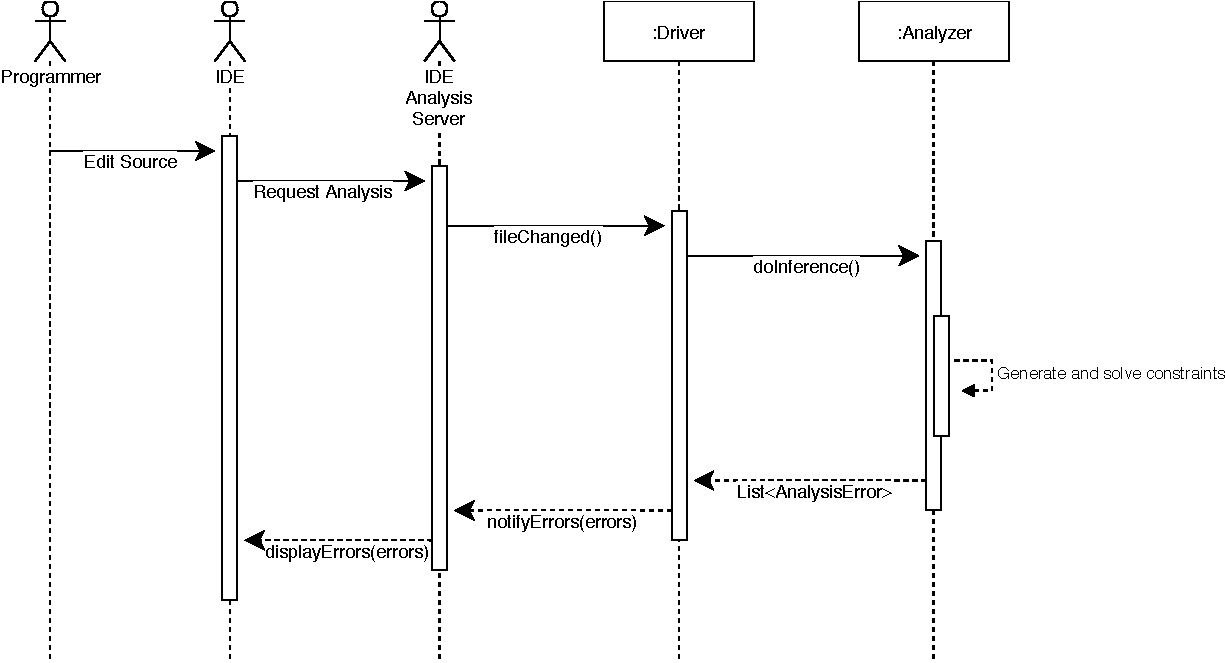
\includegraphics[width=0.8\textwidth]{images/sequence.pdf}
	\end{center}
\end{frame}

\begin{frame}[fragile]{Tipos de errores}
	\texttt{SecurityError} \\ \pause
	(código que genera una restricción inválida de esas)
\end{frame}

\begin{frame}[fragile]{Tipos de errores}
	\texttt{IllFormedTypeError} \\ \pause
	(código que posee un tipo mal formado)
\end{frame}

\begin{frame}[fragile]{Tipos de errores}
	\texttt{UndefinedFacetWarning} \\ \pause
	(Código con faceta pública no definida)
\end{frame}

\begin{frame}[fragile]{Tipos de errores}
	\texttt{InferredFacetInfo} \\ \pause
	(código con un tipo inferido)
\end{frame}

\section{Validación}

\begin{frame}[fragile]{Ejemplo: Sistema de autenticación web}
	\begin{center}
		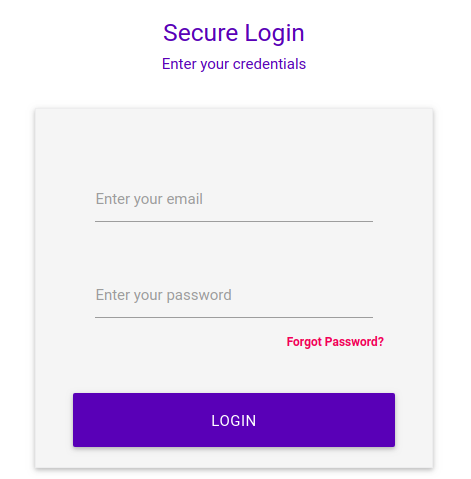
\includegraphics[width=0.5\textwidth]{images/screen4.png}
	\end{center}
\end{frame}

\begin{frame}[fragile]{Ejemplo: Sistema de autenticación web}
	(imagen en intelliJ definiendo la base de datos)
\end{frame}

\begin{frame}[fragile]{Ejemplo: Sistema de autenticación web}
	(imagen en intelliJ definiendo el metodo login)
\end{frame}

\begin{frame}[fragile]{Ejemplo: Sistema de autenticación web}
	(imagen en intelliJ mostrando la inferencia)
\end{frame}

\begin{frame}[fragile]{Ejemplo: Sistema de autenticación web}
	(imagen en intelliJ declarando una faceta pública no definida)
\end{frame}

\begin{frame}[fragile]{Ejemplo: Sistema de autenticación web}
	(imagen en intelliJ con el warning sobre la faceta no definida)
\end{frame}

\begin{frame}[fragile]{Ejemplo: Sistema de autenticación web}
	(imagen en intelliJ usando libreria html)
\end{frame}

\begin{frame}[fragile]{Ejemplo: Sistema de autenticación web}
	(imagen en intelliJ agregando Top a variable de contraseña)
\end{frame}

\begin{frame}[fragile]{Ejemplo: Sistema de autenticación web}
	(imagen en intelliJ del error de seguridad)
\end{frame}

\begin{frame}[fragile]{Ejemplo: Sistema de autenticación web}
	(imagen en intelliJ corrigiendo el error)
\end{frame}

\begin{frame}[fragile]{Ejemplo: Sistema de autenticación web}
	\begin{center}
		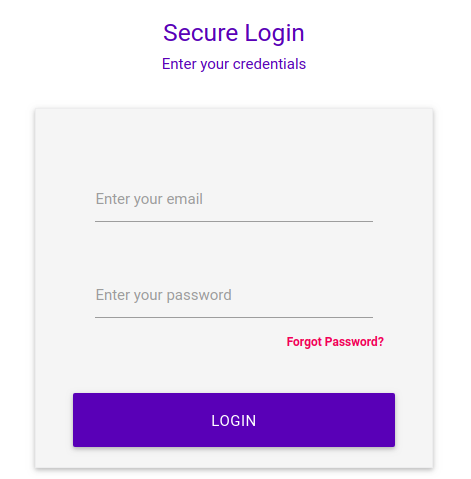
\includegraphics[width=0.5\textwidth]{images/screen4.png}
	\end{center}
\end{frame}

\begin{frame}[fragile]{Ejemplo: Sistema de autenticación web}
	\begin{table}
		\caption{Anotación de facetas públicas en identificadores}
		\begin{tabular}{c|c}
			Con inferencia & Sin inferencia\\
			\hline
			7 & 22\\
		\end{tabular}
	\end{table}
\end{frame}

\begin{frame}[fragile]{Comprobación de las reglas del sistema de tipos}
	Test unitarios en el repositorio del proyecto.
\end{frame}

\section{Conclusión}

\begin{frame}[fragile]{Conclusión}
	Conexión entre abstracciones de tipo y relaciones de orden de etiquetas de seguridad.
\end{frame}

\begin{frame}[fragile]{Trabajo futuro}
	Formalización de inferencia.
\end{frame}

\begin{frame}[fragile]{Trabajo futuro}
	Extensión al subconjunto soportado de Dart.
\end{frame}

\begin{frame}[fragile]{Trabajo futuro}
	Características de la extensión para ambientes de desarrollo.
\end{frame}

\begin{frame}[fragile]{Trabajo futuro}
	Extensión a polimorfismo. \\ \pause
	(lista parametrizada)
\end{frame}


{\setbeamercolor{palette primary}{fg=black, bg=yellow}
\begin{frame}[standout]
  Preguntas
\end{frame}
}

\appendix

\begin{frame}[fragile]{Apéndice}
  Cosas extra por posibles preguntas
\end{frame}


\end{document}
